Designovervejelser
Vi har valget at lave et program der planlægger skema for udskolingssektoren på en given skole. Vi har valgt det skal være udskoling, altså 7, 8 og 9 klasse, for at kunne simulerede at lærerne kan have klasser på tværs af klassetrinene, og der ved vise at software løsningen kan løse problemet med sammenhængene forberedelsestimer for lærerne. Derudover skal programmet kunne planlægge skemaerne således at det er muligt at have sammenlagte timer på tværs af parallel klasserne.  Da det er udskoling der arbejdes videre med, skal det specificeres hvilke parametre, der gælder for disse klassetrin. Alle klassetrinene skal undervises i dansk, idræt, matematik, engelsk, historie, biologi, geografi, fysik og kemi og sprog, derudover skal de have mulighed for at have et valgfag. For at lægge fokus på andre ting, har vi valgt at eleverne blot har et fag der hedder valgfag og alle har tysk. På syvende klassetrin er der også et praktisk fag som håndarbejde, sløjd eller hjemmekundskab på skemaet. De har til gengæld ikke kristendom på skemaet, da de har konfirmationsforberedelse.\footfullcite{lov2016} Det fulde time antal for de forskellige fag kan ses på nedenstående skema:
\begin{figure}[!h]
  \centering
  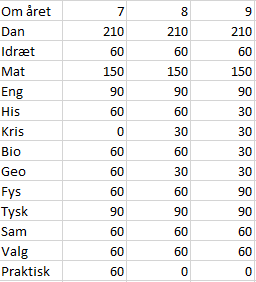
\includegraphics[width=\textwidth]{partials/graphics/antalaftimerpaaetaar.png}
  \caption{Tabel over timetallet for et år.}
  \label{fig:Timetalaar}
\end{figure}

Ugeligt vil det passe med følgende:
\begin{figure}[!h]
  \centering
  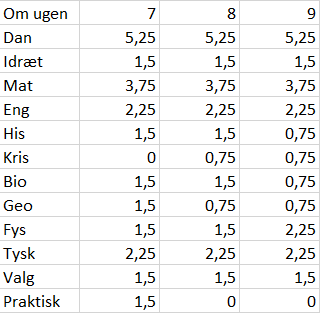
\includegraphics[width=\textwidth]{partials/graphics/antalaftimerpaaenuge.png}
  \caption{Tabel over timetallet for en uge.}
  \label{fig:Timetaluge}
\end{figure}

Derudover skal programmet opfylde de specifikke krav der bliver stillet af Sofiendalskolen. Disse krav er at alle de tunge fag, som matematik dansk og fysik/kemi, skal lægges før elevernes middagspause, da eleverne som regl er mere ukoncentrerede efter middagspausen. Sofiendalskolen vil også gerne have at lærerne har mere end en forberedelsestime adgangen. Lærerne mener at de ikke kan nå at at få lavet noget på en enkel forberedelsestime, derfor skal der helst være to eller flere forberedelsestimer ad gangen. På Sofiendalskolen vægter de også samarbejde i mellem parallel klasser højt. Skemaet skal altså lægges således at visse fag forekommer på samme tidspunkt, så samarbejde mellem klasserne er muligt.\footfullcite{interview}

Det er også vigtigt at der ikke forekommer tomme lektioner inde midt på dagen.